% Party Monopoly — Technical Design Document
% Build: pdflatex design.tex  (run twice for the table of contents / references)
\documentclass[11pt,a4paper]{article}

\usepackage[T1]{fontenc}
\usepackage[utf8]{inputenc}
\usepackage[margin=1in]{geometry}
\usepackage{lmodern}
\usepackage{microtype}
\usepackage{xcolor}
\usepackage{booktabs}
\usepackage{enumitem}
\usepackage{titlesec}
\usepackage{fancyhdr}
\usepackage{listings}
\usepackage{tikz}
\usetikzlibrary{arrows.meta,positioning,shapes.geometric}
\usepackage[hidelinks,colorlinks=true,linkcolor=accent,urlcolor=accent,citecolor=accent]{hyperref}

% ---- palette (the game's "Neon Night Market" theme) ---------------------
\definecolor{accent}{HTML}{D81B8C}     % neon magenta
\definecolor{accent2}{HTML}{1FB6C1}    % cyan
\definecolor{ink}{HTML}{1A1A22}
\definecolor{codebg}{HTML}{F5F4F8}
\definecolor{codekw}{HTML}{8E24AA}
\definecolor{codestr}{HTML}{0F8A6A}
\definecolor{codecom}{HTML}{8A8A93}

% ---- code listings ------------------------------------------------------
\lstdefinelanguage{ts}{
  keywords={interface,type,const,let,return,if,else,switch,case,default,
            readonly,number,string,boolean,null,export,import,from,class,
            extends,new,function,void,Record,Map,Promise,async,await,this},
  sensitive=true,
  morecomment=[l]{//},
  morecomment=[s]{/*}{*/},
  morestring=[b]",
  morestring=[b]'
}
\lstset{
  language=ts,
  backgroundcolor=\color{codebg},
  basicstyle=\ttfamily\footnotesize,
  keywordstyle=\color{codekw}\bfseries,
  stringstyle=\color{codestr},
  commentstyle=\color{codecom}\itshape,
  breaklines=true,
  showstringspaces=false,
  frame=single,
  rulecolor=\color{codebg},
  framesep=6pt,
  xleftmargin=4pt,
  columns=fullflexible,
  keepspaces=true
}

% ---- headings -----------------------------------------------------------
\titleformat{\section}{\Large\bfseries\color{accent}}{\thesection}{0.6em}{}
\titleformat{\subsection}{\large\bfseries\color{ink}}{\thesubsection}{0.6em}{}
\pagestyle{fancy}\fancyhf{}
\lhead{\small\textcolor{accent}{Party Monopoly}}
\rhead{\small Technical Design Document}
\cfoot{\small\thepage}
\renewcommand{\headrulewidth}{0.4pt}

% in-game currency: rendered as a glyph in the client; written "cr" in prose
\newcommand{\cur}[1]{#1\,cr}
\newcommand{\code}[1]{\texttt{#1}}

\begin{document}

% ---- title --------------------------------------------------------------
\begin{titlepage}
\centering
\vspace*{3cm}
{\Huge\bfseries\color{accent} Party Monopoly\par}
\vspace{0.4cm}
{\large\itshape Neon Night Market\par}
\vspace{1.2cm}
{\LARGE Technical Design Document\par}
\vspace{0.6cm}
{\large A deterministic Monopoly engine whose key moments break into minigames\par}
\vspace{2cm}

\begin{tikzpicture}
  \draw[accent,line width=2pt] (0,0) -- (8,0);
  \node[accent2] at (4,0.4) {\small reflex over luck};
\end{tikzpicture}
\vfill
{\small Revision 1 \quad\textbullet\quad \today\par}
\end{titlepage}

\tableofcontents
\newpage

% =========================================================================
\section{Overview}

Party Monopoly is a Monopoly variant built around one inversion of the
original game: \emph{the moments that normally resolve with arithmetic instead
resolve with a minigame.} The first version proves a single instance of this
idea, the \textbf{Rent Showdown} --- when a player lands on an opponent's
property, rent is not simply paid; the two players fight a brief two-player
reflex duel, and the result scales what the rent is worth.

This document is the technical reference for the project: the architecture, the
deterministic engine, the minigame seam, the AI, the authoritative online
server, the React client, and the economy model with its current open
questions. It is written to be read by both designers and engineers.

\subsection{Design pillars}
\begin{itemize}[leftmargin=1.4em]
  \item \textbf{Reflex over luck.} The headline mechanic rewards a skill the
        dice never test. The engine stays a faithful Monopoly skeleton so the
        twist reads as a twist.
  \item \textbf{Deterministic core.} A game is fully reproducible from its
        \code{seed} plus its action log. No wall clock and no \code{Math.random}
        ever touch the engine.
  \item \textbf{One mechanic, proven well.} The MVP ships exactly one minigame
        (Reflex Tap Duel) wired into exactly one trigger (rent). Everything
        else is a deliberately thin, faithful board.
  \item \textbf{Transport independence.} The same reducer drives hotseat,
        single-player-vs-AI, and authoritative online play. The transport
        changes; the rules do not.
\end{itemize}

\subsection{The core loop}
\begin{enumerate}[leftmargin=1.6em]
  \item Active player rolls; doubles grant another roll (three in a row sends
        them to jail).
  \item The pawn moves; passing GO pays a salary.
  \item The landed square resolves by type. Landing on an \emph{unowned}
        property offers a buy decision; landing on an \emph{opponent-owned}
        property opens a Rent Showdown.
  \item The duel decides an outcome (payer wins / owner wins / draw), which
        selects a rent multiplier. Rent is transferred; an insolvent payer goes
        bankrupt to the owner.
  \item Turn ends, the pointer advances, laps are counted, and win conditions
        are checked.
\end{enumerate}

\subsection{Build phases}
\begin{enumerate}[leftmargin=1.6em]
  \item \textbf{Engine playable in hotseat} --- the deterministic reducer and a
        local client. \emph{(complete)}
  \item \textbf{Reflex Tap Duel wired into Rent Showdown} --- the minigame seam
        and its renderer. \emph{(complete)}
  \item \textbf{Online play} --- the engine wrapped in a Colyseus room with the
        server adjudicating duels. \emph{(complete)}
\end{enumerate}

% =========================================================================
\section{Architecture}

The repository is an npm-workspaces monorepo. Six packages form a strict
dependency layering: \code{types} depends on nothing, and everything depends on
\code{types}. The engine and the minigame harness sit on top of types; the AI,
server, and web client sit on top of those.

\begin{figure}[h]
\centering
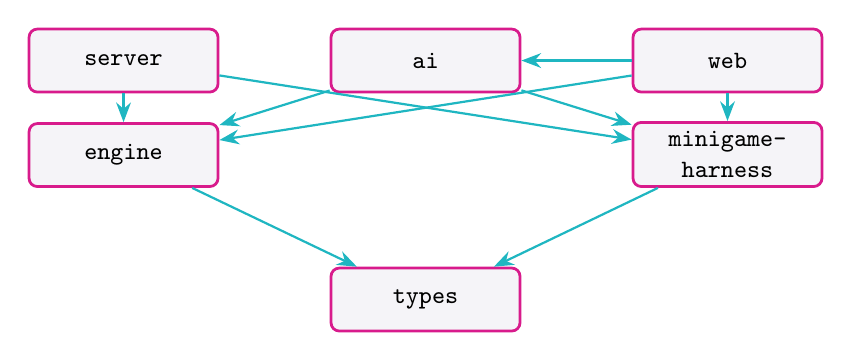
\begin{tikzpicture}[
  node distance=10mm and 14mm,
  pkg/.style={draw=accent,line width=1pt,rounded corners=3pt,fill=codebg,
              font=\ttfamily\small,minimum height=8mm,minimum width=24mm,align=center},
  dep/.style={-{Stealth[length=2.5mm]},accent2,line width=0.8pt}
]
  \node[pkg] (types) {types};
  \node[pkg,above left=of types] (engine) {engine};
  \node[pkg,above right=of types] (mh) {minigame-\\harness};
  \node[pkg,above=22mm of types] (ai) {ai};
  \node[pkg,left=of ai] (server) {server};
  \node[pkg,right=of ai] (web) {web};

  \draw[dep] (engine) -- (types);
  \draw[dep] (mh) -- (types);
  \draw[dep] (ai) -- (engine);
  \draw[dep] (ai) -- (mh);
  \draw[dep] (server) -- (engine);
  \draw[dep] (server) -- (mh);
  \draw[dep] (web) -- (engine);
  \draw[dep] (web) -- (mh);
  \draw[dep] (web) -- (ai);
\end{tikzpicture}
\caption{Package dependency graph. Arrows point from dependent to dependency.}
\end{figure}

\begin{table}[h]
\centering
\small
\begin{tabular}{@{}lll@{}}
\toprule
\textbf{Package} & \textbf{Role} & \textbf{Depends on} \\
\midrule
\code{types}             & Branded ids, action/event/minigame/wire types & --- \\
\code{engine}            & Pure deterministic reducer, board, RNG, tunables & types \\
\code{minigame-harness}  & Minigame interface, registry, reflex adjudication & types \\
\code{ai}                & Deterministic bot decisions and duel reflexes & engine, harness \\
\code{server}            & Authoritative Colyseus room wrapping the engine & engine, harness \\
\code{sim}               & Headless bot-vs-bot balance simulation & engine, harness, ai \\
\code{apps/web}          & React + Vite client, Zustand state mirror & engine, harness, ai \\
\bottomrule
\end{tabular}
\caption{Packages and their dependencies.}
\end{table}

\subsection{Source-as-entry workspaces}
Each package's \code{package.json} points \code{main} and \code{types} directly
at \code{./src/index.ts}. Consumers resolve TypeScript source straight from the
workspace, so no per-package build step is needed during development. Workspace
dependencies are pinned with \code{"*"}.

\subsection{TypeScript project setup}
A shared \code{tsconfig.base.json} enforces a strict suite: \code{strict},
\code{noUncheckedIndexedAccess}, \code{noImplicitOverride},
\code{noFallthroughCasesInSwitch}, \code{noImplicitReturns},
\code{exactOptionalPropertyTypes}, \code{isolatedModules}, and
\code{verbatimModuleSyntax}, targeting ES2022 with \code{composite} incremental
builds. The root \code{tsconfig.json} is a solution file referencing
\code{types}, \code{engine}, \code{minigame-harness}, \code{ai}, and \code{web}.
The \code{server} is intentionally \emph{not} referenced --- it builds
independently under \code{NodeNext} module resolution because it is a Node
application rather than a bundled library.

% =========================================================================
\section{The Engine}

The engine is pure TypeScript with no React, no DOM, no wall clock, and no
\code{Math.random}. Its barrel (\code{packages/engine/src/index.ts}) re-exports
the RNG, tunables, state, actions, events, board, init, and reducer.

\subsection{Determinism}
Randomness lives \emph{inside} game state as a serializable \code{RngState}. The
generator is a seeded mulberry32 (\code{rng.ts}); each draw returns both a value
and the \emph{next} state, which the caller stores back into \code{GameState}.
Because the only source of entropy is \code{state.rng}, a game replays exactly
from \code{seed} plus its ordered action log. The UI and server are free to use
the wall clock (\code{performance.now()}, \code{Date.now()}, \code{Math.random}
for timing jitter) because none of that crosses the engine boundary.

\subsection{Game state}
\begin{lstlisting}
interface GameState {
  seed: number;
  rng: RngState;
  tunables: GameTunables;
  board: readonly Square[];
  players: readonly PlayerState[];
  activePlayerIndex: number;            // index into players
  phase: TurnPhase;
  ownership: Record<number, PlayerId>;  // squareId -> owner; missing = buyable
  lastRoll: readonly number[] | null;
  doublesCount: number;                 // 3 in a row -> jail; reset each turn
  round: number;                        // laps; roundCap force-ends the game
  pendingMinigame: MinigameRequest | null;
  winnerId: PlayerId | null;
}
\end{lstlisting}

A \code{PlayerState} carries \code{id, name, isAI, money, position, inJail,
jailTurns, bankrupt}. A \code{Square} is \code{id, name, type} with optional
\code{PropertyData} (\code{price, baseRent, group}).

\subsection{Turn phases}
The \code{TurnPhase} union is:
\begin{quote}\ttfamily\small
AWAITING\_ROLL $\to$ MOVING $\to$ RESOLVING\_SQUARE $\to$\\
AWAITING\_BUY\_DECISION | RENT\_SHOWDOWN $\to$ TURN\_END $\to$ GAME\_OVER
\end{quote}
\code{MOVING} and \code{RESOLVING\_SQUARE} are transient labels --- the reducer
threads straight through them and never rests there. The two phases the engine
genuinely \emph{parks} on are \code{RENT\_SHOWDOWN} (waiting for a minigame
result) and \code{GAME\_OVER} (terminal). \code{AWAITING\_BUY\_DECISION} and
\code{TURN\_END} await a player action.

\begin{figure}[h]
\centering
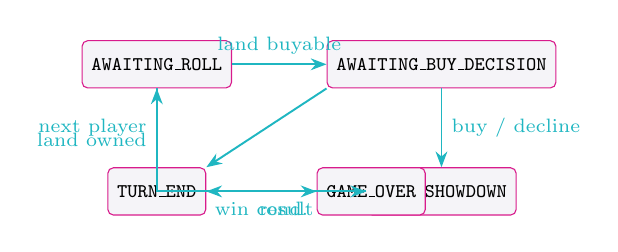
\begin{tikzpicture}[
  node distance=7mm and 12mm,
  st/.style={draw=accent,rounded corners=2pt,fill=codebg,font=\ttfamily\scriptsize,
             minimum height=6mm,align=center},
  fl/.style={-{Stealth[length=2mm]},accent2,line width=0.7pt,font=\scriptsize}
]
  \node[st] (roll) {AWAITING\_ROLL};
  \node[st,right=of roll] (buy) {AWAITING\_BUY\_DECISION};
  \node[st,below=10mm of buy] (show) {RENT\_SHOWDOWN};
  \node[st,below=10mm of roll] (end) {TURN\_END};
  \node[st,right=14mm of end] (over) {GAME\_OVER};

  \draw[fl] (roll) -- node[above]{land buyable} (buy);
  \draw[fl] (roll) |- node[pos=0.25,left]{land owned} (show);
  \draw[fl] (buy) -- node[right]{buy / decline} (show.north);
  \draw[fl] (buy.south west) -- (end.north east);
  \draw[fl] (show) -- node[below]{result} (end);
  \draw[fl] (end) -- node[below]{win cond.} (over);
  \draw[fl] (end.north) -- node[left]{next player} (roll.south);
\end{tikzpicture}
\caption{Phase transitions the engine actually rests on (transient
\code{MOVING}/\code{RESOLVING\_SQUARE} elided).}
\end{figure}

\subsection{Actions and events}
Actions are the only way to mutate state. The set is:
\begin{lstlisting}
type GameAction =
  | { type: "ROLL_DICE" }
  | { type: "BUY_PROPERTY" }
  | { type: "DECLINE_BUY" }
  | { type: "PAY_JAIL_FINE" }
  | { type: "SUBMIT_MINIGAME_RESULT"; result: MinigameResult }
  | { type: "END_TURN" }
  | { type: "DECLARE_BANKRUPT"; playerId: PlayerId };
\end{lstlisting}

The reducer is a pure \code{reduce(state, action)} returning
\code{\{ state, events \}}. Emitted events --- \code{DICE\_ROLLED},
\code{PLAYER\_MOVED}, \code{PROPERTY\_BOUGHT}, \code{MINIGAME\_REQUESTED},
\code{RENT\_PAID}, \code{SENT\_TO\_JAIL}, \code{PLAYER\_BANKRUPT},
\code{TURN\_ENDED}, \code{GAME\_OVER} --- let clients react (animate, log
telemetry, count showdowns) without re-deriving state.

\subsection{Square resolution and the rent flow}
Landing dispatches by square type. \code{GO\_TO\_JAIL} jails the player; tax
deducts \code{taxAmount}; \code{CHANCE} and \code{COMMUNITY} are deliberately
inert and resolve like Free Parking in the MVP. A property landed on:
\begin{itemize}[leftmargin=1.4em,nosep]
  \item \textbf{unowned} $\to$ phase \code{AWAITING\_BUY\_DECISION};
  \item \textbf{owned by the lander} $\to$ nothing;
  \item \textbf{owned by an opponent} $\to$ a Rent Showdown is opened.
\end{itemize}
Opening a showdown builds a \code{MinigameRequest} whose participants are
ordered \textbf{[payer (index 0), owner (index 1)]}, parks the phase at
\code{RENT\_SHOWDOWN}, and emits \code{MINIGAME\_REQUESTED}. This
\textbf{payer-is-0, owner-is-1 ordering is load-bearing} and assumed everywhere
downstream (rent multiplier resolution, server adjudication, the client's
AI-seat detection).

\subsection{Win conditions}
On \code{END\_TURN} the engine checks, in order:
\begin{enumerate}[leftmargin=1.6em,nosep]
  \item \textbf{Last player standing.} If at most one solvent player remains,
        that player wins.
  \item \textbf{Lap counting.} When the turn pointer wraps back to the first
        solvent player, \code{round} increments.
  \item \textbf{Round cap.} If \code{roundCap > 0} and \code{round} exceeds it,
        the game force-ends and the \emph{richest} player wins by the
        configured \code{tiebreakMetric}.
\end{enumerate}
\code{netWorth} is cash plus the price of owned properties, unless the tiebreak
metric is \code{"CASH"} (cash only). The round cap exists so a game always
terminates --- see the economy section for why that matters today.

% =========================================================================
\section{The Minigame Harness}

The harness is the seam that makes the minigame swappable across transports. It
is renderer-agnostic --- no DOM imports --- so the same adjudication code runs
in the browser and on the server.

\subsection{Interface and registry}
\begin{lstlisting}
interface Minigame {
  id: MinigameId;
  minPlayers: number;
  maxPlayers: number;
  play(request: MinigameRequest): Promise<MinigameResult>;
}
\end{lstlisting}
A \code{Minigame} must always resolve --- on failure it returns status
\code{ABORTED} rather than rejecting. The \code{MinigameRegistry} maps ids to
implementations (\code{register} throws on duplicates) and \code{run(request)}
resolves a request end-to-end. This registry is where hotseat, AI, and online
modes swap implementations in.

\subsection{Reflex Tap Duel}
The shared contract lives in \code{reflex-tap-duel.ts}; the actual renderer is
in the web client. Configuration:
\begin{lstlisting}
const DEFAULT_REFLEX_TAP_DUEL_CONFIG = {
  minDelayMs: 1500,        // earliest the "go" can appear
  maxDelayMs: 4000,        // latest the "go" can appear
  drawWindowMs: 25,        // reactions within this gap are a draw
  minHumanReactionMs: 100, // faster than this is treated as anticipation
};
\end{lstlisting}

\subsection{Adjudication}
\code{adjudicateReflexDuel(p0, p1, payerId, ownerId, drawWindowMs)} is pure and
exhaustive over the edge cases (with \code{p0 = payer}, \code{p1 = owner}):
\begin{itemize}[leftmargin=1.4em,nosep]
  \item both false-start $\to$ \code{ABORTED};
  \item exactly one false-start $\to$ the other player wins;
  \item both reactions null (no tap) $\to$ \code{ABORTED};
  \item exactly one null $\to$ the player who tapped wins;
  \item reaction gap $\le$ \code{drawWindowMs} $\to$ \code{DRAW};
  \item otherwise the faster reaction wins.
\end{itemize}
The result is a \code{MinigameResult} (\code{minigameId, status, outcome,
ranking, metrics}) carrying \code{P0\_WIN | P1\_WIN | DRAW} and \code{COMPLETED
| ABORTED}. The guiding principle of the whole seam:
\emph{the minigame decides who won; the engine decides what that win is worth.}

% =========================================================================
\section{The AI}

The AI package is pure and deterministic --- it does not call the engine's RNG,
and its only nondeterminism (duel reflexes) takes an injectable random source
so tests can pin it.

\subsection{Turn decisions}
\code{decideAction(state, playerId)} returns the next \code{GameAction} or
\code{null} when it is not this bot's turn (or the game is in a showdown or
over). The policy is intentionally simple:
\begin{itemize}[leftmargin=1.4em,nosep]
  \item \code{AWAITING\_ROLL}: if jailed and the fine is affordable, pay it;
        otherwise roll.
  \item \code{AWAITING\_BUY\_DECISION}: buy when \code{price <= money * 0.6}
        (the \code{BUY\_CASH\_FRACTION} guard), else decline.
  \item \code{TURN\_END}: end the turn.
\end{itemize}
Notably the AI never returns \code{SUBMIT\_MINIGAME\_RESULT} --- the host drives
the duel and feeds the result back.

\subsection{Duel reflexes}
\code{aiReflexInput(skill, rng)} produces a \code{ReflexInput} for a bot seat.
False-start probability is \code{0.12 * (1 - skill)}; reaction mean is
\code{600 - 350 * skill} milliseconds with up to $\pm$60\,ms of jitter, floored
at 250\,ms. A \code{skill} of 0.6 is the default opponent, landing a believable
human-ish reaction band.

% =========================================================================
\section{The Online Server}

The server wraps the engine in a Colyseus room and is fully
\textbf{authoritative}: clients send intents and taps, never results. It listens
on \code{PORT} (default 2567) and defines a single \code{"game"} room with
\code{maxClients = 2}.

\subsection{Room lifecycle}
\code{GameRoom} holds the \code{GameState}, a seat map
(\code{sessionId $\to$ PlayerId}), per-seat taps, and timers. The first two
joiners take seats \code{p0} and \code{p1}; the game starts (seeded with
\code{Date.now()}) once both are present. A consented leave ends the room; a
network drop opens a 30-second reconnection window, after which the server
re-sends state to the returning client.

\subsection{Action handling and the legality gate}
Incoming actions pass through \code{isLegalAction(state, playerId, action)}
before reaching the reducer. Where the reducer silently no-ops an illegal
action (fine for local play), the online path must \emph{reject} it with an
error message, so \code{validate.ts} mirrors the reducer's guards: no actions in
\code{GAME\_OVER}/\code{RENT\_SHOWDOWN}, only on your turn, only when not
bankrupt, and each action only in its proper phase. Legal actions are reduced
and the new state is broadcast; if the phase becomes \code{RENT\_SHOWDOWN}, the
server starts a showdown.

\subsection{Server-run showdown}
\begin{enumerate}[leftmargin=1.6em,nosep]
  \item \textbf{start} --- taps are cleared and \code{showdown:start} is
        broadcast with the property's \code{baseRent}.
  \item \textbf{go} --- after a randomized delay (\code{minDelayMs} plus a
        random span up to \code{maxDelayMs}), \code{showdown:go} is broadcast
        and a 5-second tap timeout is armed.
  \item \textbf{tap} --- each seat may submit one tap; once both arrive (or the
        timeout fires, filling absentees with a \code{MISSING\_TAP}) the
        showdown resolves.
  \item \textbf{resolve} --- \code{adjudicateShowdown} sanitizes both taps,
        adjudicates via the harness, and the result is fed back through the
        reducer as \code{SUBMIT\_MINIGAME\_RESULT}. New state is broadcast.
\end{enumerate}
\textbf{Anti-cheat:} \code{sanitizeTap} demotes any non-false-start reaction
faster than \code{minHumanReactionMs} (100\,ms) to a false start, so a client
cannot "win" by anticipating or spoofing an impossibly fast tap. Crucially, the
client wire protocol's \code{ClientActionType} omits
\code{SUBMIT\_MINIGAME\_RESULT} entirely --- the result type a client could forge
is simply not part of the messages it is allowed to send.

\subsection{Wire protocol}
Client-to-server (\code{C2S}) carries \code{action} and \code{tap} messages.
Server-to-client (\code{S2C}) carries \code{state} (a generic
\code{StateMessage} with the player's own id, kept generic so \code{types} need
not depend on \code{engine}), \code{showdown:start}, \code{showdown:go}, and
\code{error}. Tap timing is measured \emph{client-side from receipt of the "go"
signal}, not from any shared wall clock, which keeps latency from biasing the
duel.

% =========================================================================
\section{The Web Client}

The client is React + Vite with Zustand for state. The store \emph{mirrors}
engine state rather than replacing it: the engine's \code{GameState} remains the
source of truth, and the store pipes every dispatch through the real
\code{reduce()}.

\subsection{Modes}
\code{App.tsx} is a mode switcher: \code{menu}, \code{hotseat}, \code{ai}
(hotseat reused with a bot seat), \code{duel} (a board-less fairness practice),
and \code{online}.

\subsection{Components}
\begin{itemize}[leftmargin=1.4em]
  \item \textbf{Board} --- 40 squares on an 11$\times$11 CSS-grid ring, GO at
        bottom-right, counter-clockwise. Eight district colors, owner-inset
        borders, pawns, and a center panel showing round and phase.
  \item \textbf{Hud} --- phase, round, last roll, and per-player cards (money,
        position, jail/bankrupt status).
  \item \textbf{ReflexTapDuel} --- the hotseat (one-keyboard) duel: payer taps
        \code{A}, owner taps \code{L}; red arms to green after a randomized
        delay; a bot seat can be sampled up front. Measures with
        \code{performance.now()}.
  \item \textbf{OnlineReflexDuel} --- the single-seat, server-driven duel: red
        on "start", green on "go", tap on Space/Enter, then wait for the
        authoritative result.
  \item \textbf{DuelSignal} --- the shared red/green visual, deliberately
        colorblind-safe: shape, glyph, text, and \code{aria-label} all change,
        not just hue.
  \item \textbf{HotseatGame / OnlineGame} --- the two game shells, dispatching
        through the reducer or through \code{sendAction} respectively.
  \item \textbf{DuelPractice} --- a board-less "Phase 0 fairness gate" running
        duels back-to-back with a scoreboard (win rate, average reaction, false
        starts, draws).
  \item \textbf{DebugPanel} --- a dev-only panel (hotseat/practice) to restart
        with a seed, teleport the active player, or set money via a local
        \code{debugPatch} that bypasses the reducer.
\end{itemize}

\subsection{Stores and telemetry}
\code{gameStore} holds the mirrored state, the AI seat/skill (\code{p1} at skill
0.6), a showdown counter derived from \code{MINIGAME\_REQUESTED} events, and a
duel log. \code{onlineStore} tracks connection status
(\code{idle/connecting/waiting/playing/reconnecting/error/left}) and a
\code{showdown} signal whose \code{seq} field bumps on each phase change to
disambiguate a stale "start" from a fresh "go". \code{net/onlineClient} is a
thin, React-free wrapper over \code{colyseus.js} that stores the reconnection
token and maps each server message to a handler. \code{telemetry/duel} flattens
each result into a serializable \code{DuelRecord} and aggregates win rates and
average reaction (over non-false-start taps only) --- the data behind the
fairness gate.

% =========================================================================
\section{Economy and Tuning}

\subsection{Default tunables}
\begin{lstlisting}
const DEFAULT_TUNABLES = {
  startingMoney: 1200,
  passGoSalary:  75,
  taxAmount:     120,
  boardSize:     40,
  diceCount:     2,
  diceSides:     6,
  jail: { jailSquareId: 10, fine: 50, maxTurns: 3, releaseOnDoubles: true },
  rentMultipliers: { ownerWin: 1.5, payerWin: 0.5, draw: 1.0, aborted: 1.0 },
  rentFraction:  0.2,    // baseRent = max(rentFloor, floor(price * 0.2))
  rentFloor:     8,
  rentEscalationStep: 0,  // off by default; held for a playtest pass
  rentEscalationCap:  4,
  roundCap:      30,
  tiebreakMetric: "NET_WORTH",
};
\end{lstlisting}

\subsection{How rent is priced}
A property's \code{baseRent} is computed \emph{once at board build} as
\code{max(rentFloor, floor(price * rentFraction))} --- 20\% of price, floored at
8. At showdown time the duel outcome selects a multiplier (owner win
$\times$1.5, payer win $\times$0.5, draw $\times$1.0, aborted $\times$1.0) and
the payment is \code{round(baseRent * multiplier * escalation)}. If the payer
cannot cover it, they pay all their cash and go bankrupt to the owner.

The \code{escalation} factor stands in for the missing houses and hotels: rent
climbs with how many properties the owner holds, as
\code{min(rentEscalationCap, 1 + rentEscalationStep * (owned - 1))} --- a lone
property never escalates, and the factor is capped. With
\code{rentEscalationStep = 0} (the default) the factor is always 1, so rent is
unescalated until a playtest decides the value.

\subsection{The convergence problem}
The MVP cut houses and hotels. In real Monopoly those are what scale rent
steeply enough to bankrupt players; without them, flat rent plus the modest
$0.5\times$--$1.5\times$ duel multiplier produces rents that stay small relative
to recurring income. A bot-vs-bot simulation under the original tunables
(\code{startingMoney 1500}, \code{passGoSalary 200}, flat low rents) showed
\textbf{9 of 10 games never reaching \code{GAME\_OVER}} --- every player's net
worth only grew, so nobody went bankrupt and the last-player-standing condition
could never fire. The cause was confirmed to be tunables, not a bug: a punitive
re-run (low salary, high tax, low starting money) finished 10/10 games.

\subsection{The interim fix (shipped)}
The current defaults above are the response: lower starting money and pass-GO
salary, rent raised to 20\% of price (now driven by the \code{rentFraction} /
\code{rentFloor} tunables), and a \code{roundCap} of 30 with a
\code{tiebreakMetric} of \code{NET\_WORTH} that force-ends a stalled game to the
richest player. Under these, the simulation finishes \textbf{30 of 30 games,
median $\approx$62 turns.}

\subsection{Measuring convergence --- the sim harness}
Balance is now measured by a committed, headless bot-vs-bot harness
(\code{packages/sim}), so the convergence question is data rather than anecdote.
It drives the real engine with the real AI and seeded reflex duels --- fully
deterministic from a seed --- and classifies each game's ending as
\emph{elimination} (a last-player-standing win), \emph{cap} (the round cap
force-ended it on net worth), or \emph{timeout} (never resolved within the step
guard --- a balance smell). Run it with \code{npm run sim} (e.g.\
\code{-{}-games 300 -{}-players 4 -{}-escalation 0.5}).

The harness reproduces the historical 2-player baseline exactly
(26.7\% elimination), which validates it against the earlier ad-hoc runs. It
also reveals that player count matters more than previously recorded: with the
shipped defaults, a 2-player game eliminates 26.7\% of the time, but a 4-player
game almost never does (0.7\%) --- spreading wealth across four players keeps
flat rent from bankrupting anyone, so nearly every 4-player game ends on the cap.

\begin{table}[h]
\centering
\small
\begin{tabular}{@{}llrrr@{}}
\toprule
\textbf{Players} & \textbf{Escalation} & \textbf{Elimination} & \textbf{Cap} & \textbf{Median turns} \\
\midrule
2 & off (step 0)        & 26.7\% & 73.3\% & 54 \\
2 & step 0.5, cap 4     & 84.0\% & 16.0\% & 37 \\
4 & off (step 0)        &  0.7\% & 99.3\% & 87 \\
4 & step 0.5, cap 4     & 53.0\% & 47.0\% & 72 \\
4 & step 1.0, cap 5     & 80.3\% & 19.7\% & 58 \\
\bottomrule
\end{tabular}
\caption{Ending mix over 300 seeds per row (skill 0.6). All rows finish 100\%
of games; escalation moves wins from the cap toward bankruptcy elimination.}
\end{table}

\subsection{Open question --- elimination vs. points}
Rent escalation is now \emph{implemented} (the \code{rentEscalationStep} /
\code{rentEscalationCap} tunables above) but ships \textbf{off}, so the default
balance is unchanged and games still mostly end on the cap. The data shows the
lever works: \code{step 0.5, cap 4} lifts 4-player elimination from 0.7\% to
53\%, and a steeper \code{step 1.0, cap 5} reaches 80\%. What remains is a
\emph{feel} decision --- how often a game should end by knocking someone out
versus on points, and at what player count --- which is a playtest call, not a
code one. QA has flagged a prerequisite: the reflex-duel's \emph{fairness}
should be validated with a short human, duel-only session (the Phase 0 fairness
gate / \code{DuelPractice} mode) \emph{before} committing an escalation value ---
there is no point tuning the stakes of a duel that does not yet feel fair.

% =========================================================================
\section{Building, Testing, Running}

\subsection{Scripts}
From the repository root:
\begin{lstlisting}
pnpm install
pnpm dev          // apps/web dev server
pnpm build        // apps/web production build
pnpm typecheck    // tsc across workspaces (--if-present)
pnpm test         // vitest across workspaces (--if-present)
pnpm sim          // headless balance simulation (see Economy)
pnpm lint         // eslint .
\end{lstlisting}
The server and the sim run independently with \code{tsx}; neither is a bundled
library, so both use \code{NodeNext} resolution and are left out of the root
TypeScript solution's project references.

\subsection{Tests}
Vitest suites cover the load-bearing pure logic: engine determinism and game
logic, AI decisions and reflexes, reflex adjudication, and the server's showdown
sanitization and action legality. The web client has no automated tests yet ---
its behavior is exercised through the fairness-gate playtest mode instead.

\begin{table}[h]
\centering
\small
\begin{tabular}{@{}ll@{}}
\toprule
\textbf{Package} & \textbf{Test files} \\
\midrule
engine            & \code{determinism.test.ts}, \code{game-logic.test.ts} \\
ai                & \code{decide.test.ts}, \code{reflex.test.ts} \\
minigame-harness  & \code{reflex-adjudicate.test.ts} \\
server            & \code{showdown.test.ts}, \code{validate.test.ts} \\
sim               & \code{simulate.test.ts} (determinism, termination, escalation) \\
\bottomrule
\end{tabular}
\caption{Current automated test coverage.}
\end{table}

\subsection{Reproducing a game}
Because the engine is deterministic, a bug report needs only the \code{seed} and
the action log. Replaying those through \code{reduce()} reconstructs the exact
state at any step --- the same property the bot-vs-bot economy simulations rely
on, and the reason the determinism boundary is guarded so strictly.

% =========================================================================
\section{Glossary}
\begin{description}[leftmargin=0pt,style=nextline]
  \item[Rent Showdown] The reflex duel triggered by landing on an
        opponent-owned property; its outcome scales the rent.
  \item[Tunables] The data-driven economy parameters (\code{DEFAULT\_TUNABLES})
        that configure money, rent, jail, and win conditions without code
        changes.
  \item[Round cap] A lap limit (default 30) that force-ends a stalled game to
        the richest player, guaranteeing termination.
  \item[Participant ordering] The load-bearing convention that minigame
        participant index 0 is the payer/lander and index 1 is the owner.
  \item[Determinism boundary] The rule that only the engine's seeded RNG may
        affect game state; the UI and server may use the wall clock freely.
  \item[Authoritative server] The model where the server alone adjudicates
        duels and submits results; clients send only intents and taps.
\end{description}

\end{document}
